   % Pr�sentation-Vorlage Universit�t T�bingen
% erstellt von Ekaterina Kohler (ekaterina.kohler@googlemail.com)
\documentclass[20pt,t,xcolor=table]{beamer}
\usepackage{praesentation}
\usepackage[linguistics]{forest}
\usepackage{gb4e}
\usepackage{tipa}
\let\eachwordone=\sffamily %or \normalfont
\let\eachwordtwo=\sffamily


%-------------!!!!BITTE AUSF�LLEN!!!!------------------
% hier f�ngt die Eingabe der Grundinformationen zur Pr�sentation an
\newcommand{\fakult}{Faculty of Philosophy}	%Fakult�t
\newcommand{\fbname}{General Linguistics} %Fachbereich oder Name des Instituts
\newcommand{\fussnote}{Semantics \& Pragmatics, SoSe 2021, Bentz} %Text der Fusszeile auf den Innenfolien
\newcommand{\crtext}{\copyright\ 2012 Universit�t T�bingen } %Copyright-Text
%\newcommand{\kooplogoUnten}{\colorbox{cyan}{\parbox{0.2\textwidth}{\centering \fontsize{12pt}{12pt}\selectfont MAX. ZWEI externe Koop.-Logos}}} %Kooperations-Logo in der Fusszeile auf der Titelseite. Statt \colorbox MAX. ZWEI externe Koop.-Logos. Falls kein Koop.-Logo verwendet werden soll, lassen Sie die zweite geschweifte Klammer leer

%change colour of sections and subsections in table of contents


\begin{document}

\begin{frame} %Titelseite
\author{Christian Bentz} %Autor/Verfasser
\title{Semantics \& Pragmatics SoSe 2021} %Titel
\subtitle{Lecture 2: Information Theory I} %Untertitel
\date{29/04/2021} %Datum
\newcommand{\titelbild}{{\color{grau}\rule{\textwidth}{70mm}}\\[-0.4cm]{\color{rot}\rule{\textwidth}{5mm}}} %statt grauer Box ein Deckblattbild einf�gen und die rote Linie nach oben versetzen, hier um 0.35cm
\maketitle \\
\vspace*{35mm} %Abstand zwischen dem Untertitel und Datum/Verfasser. Hier 35mm
{\fontsize{16}{16}\selectfont\bf\insertdate , \insertauthor} \hfill %\kooplogoUnten
\end{frame}

{
\setbeamertemplate{sidebar right}{}
\begin{frame}
\frametitle{Overview} 
  \tableofcontents
\end{frame}
}

\section{Section 1: Historical Overview}

%Section beginning slide
{
\setbeamertemplate{sidebar right}{}
\begin{frame}
\title{Section 1: Historical Overview} %Titel
\newcommand{\titelbild}{{\color{grau}\rule{\textwidth}{70mm}}\\[-0.4cm]{\color{rot}\rule{\textwidth}{5mm}}} %statt grauer Box ein Deckblattbild einf�gen und die rote Linie nach oben versetzen, hier um 0.35cm
\maketitle
\end{frame}
}

\begin{frame}{A Brief History of Information and Language}
    \begin{columns}[T]
        \begin{column}{6cm}
        \includegraphics[width=1\textwidth]{img/shannon4.jpg}
        \end{column}
        \begin{column}{10cm}
        \small
        \textit{The fundamental problem of communication is that of reproducing at one point either exactly or approximately a message selected at another point. [...] \textbf{semantic aspects of communication are irrelevant to the engineering problem}. The significant aspect is that the actual message is one selected from a set of possible messages.}\\
        \vspace{0.5cm}
        \footnotesize{\color{gray} Shannon, Claude E. (1948). A mathematical theory of communication, p. 1.}
        \end{column}
    \end{columns}
\end{frame}

\begin{frame}{Example}
\texttt{Article 1\\ All human beings are born free and equal in dignity and rights. They are endowed with reason and conscience and should act towards one another in a spirit of brotherhood.}\\
\vspace{0.2cm}
\small
Universal Declaration of Human Rights (UDHR) in English\\
\vspace{0.5cm}
\normalsize
\texttt{Raeiclt 1\\
      Rll humrn btings rat boan fatt and tqurl in digniey rnd aighes. Ehty rat tndowtd wieh atrson rnd conscitnct rnd should rce eowrads ont rnoehta in r spiaie of baoehtahood.}
\\
\vspace{0.2cm}
\small
Universal Declaration of Human Rights (UDHR) in ???\\
\end{frame}

\begin{frame}{A Brief History of Information and Language}
    \begin{columns}[T]
        \begin{column}{6cm}
        \includegraphics[width=1\textwidth]{img/shannon4.jpg}\\
        \vspace{0.2cm}
        \includegraphics[width=1\textwidth]{img/weaver.jpg}
        \end{column}
        \begin{column}{10cm}
        \small
        \textit{[...] two messages, one of which is heavily loaded with meaning and the other which is pure nonsense, can be exactly equivalent, from the present viewpoint, as regards information. It is this, undoubtedly, that Shannon means when he says that ``the semantic aspects of communication are irrelevant to the engineering aspects.'' \textbf{But this does not mean that the engineering aspects are necessarily irrelevant to the semantic aspects}.}\\
        \vspace{0.5cm}
        \footnotesize{\color{gray} Shannon \& Weaver (1949). The mathematical theory of communication, p. 8.}
        \end{column}
    \end{columns}
\end{frame}

\begin{frame}{Three Levels of Communication Problems}
    \begin{columns}[T]
        \begin{column}{6cm}
        \includegraphics[width=1\textwidth]{img/shannon4.jpg}\\
        \vspace{0.2cm}
        \includegraphics[width=1\textwidth]{img/weaver.jpg}
        \end{column}
        \begin{column}{10cm}
        \small
        \begin{itemize}
        \item \textbf{Level A}: How accurately can the symbols of communication be transmitted? (The technical problem.)
        \item \textbf{Level B}: How precisely do the transmitted symbols convey the desired meaning? (The semantic problem.)
        \item \textbf{Level C}: How effectively does the received meaning affect conduct in the desired way? (The effectiveness problem.)
        \end{itemize}
        \vspace{0.5cm}
        \footnotesize{\color{gray} Shannon \& Weaver (1949). The mathematical theory of communication, p. 4.}
        \end{column}
    \end{columns}
\end{frame}

\begin{frame}{A Brief History of Information and Language}
    \begin{columns}[T]
        \begin{column}{6cm}
        \includegraphics[width=1\textwidth]{img/harris.jpg}\\
        \includegraphics[width=1\textwidth]{img/harrisBook.jpg}
        \end{column}
        \begin{column}{10cm}
        \small
        \textit{\textbf{The theory of syntax is stated in terms related to mathematical Information Theory: as constraints on word combination}, each later constraint being defined on the resultants of a prior one. This structure not only permits a finitary description of the unbounded set of sentences, but also admits comparison of language with other notational systems, [...]}\\
        \vspace{0.5cm}
        \footnotesize{\color{gray} Harris, Zellig (1991). A theory of language and information. A mathematical approach.}
        \end{column}
    \end{columns}
\end{frame}

\begin{frame}{A Brief History of Information and Language}
    \begin{columns}[T]
        \begin{column}{6cm}
        \includegraphics[width=1\textwidth]{img/chomsky.jpg}
        \end{column}
        \begin{column}{10cm}
        \small
        \textit{[...] To complete this elementary communication theoretic model for language, we assign a probability to each transition from state to state. We can then calculate the "uncertainty" associated with each state and we can define the "information content" of the language as the average uncertainty, weighted by the probability of being in the associated states. \textbf{Since we are studying grammatical, not statistical structure of language here, this generalization does not concern us.}}\\
        \vspace{0.2cm}
        \footnotesize{\color{gray} Chomsky, Noam (1957). Syntactic Structures, p. 20.}
        \end{column}
    \end{columns}
\end{frame}

\section{Section 2: Introduction}

{
\setbeamertemplate{sidebar right}{}
\begin{frame}
\title{Section 2: Introduction} %Titel
\newcommand{\titelbild}{{\color{grau}\rule{\textwidth}{70mm}}\\[-0.4cm]{\color{rot}\rule{\textwidth}{5mm}}} %statt grauer Box ein Deckblattbild einf�gen und die rote Linie nach oben versetzen, hier um 0.35cm
\maketitle
\end{frame}
}

\begin{frame}{What's the difference?}
\vspace{0.5cm}
\begin{columns}
\begin{column}{5cm}
\centering \includegraphics[width=1.2\textwidth]{img/bug.jpg}\\
\vspace{0.2cm}
\centering \includegraphics[width=1.2\textwidth]{img/leaf.jpg}
\end{column}
\begin{column}{7cm}
\centering \includegraphics[width=1.2\textwidth]{img/paleoSign7.png}\\
\vspace{0.2cm}
\centering \includegraphics[width=1.2\textwidth]{img/sumerian2.jpg}
\end{column}
\end{columns}
\end{frame}

\subsection{}
\begin{frame}{Some Intuitive Terminology}
\begin{columns}[T]
\begin{column}{12cm}
\begin{itemize}
\item order $\leftrightarrow$ disorder
\item regularity $\leftrightarrow$ irregularity
\item predictability $\leftrightarrow$ unpredictability
\item certainty $\leftrightarrow$ uncertainty
\item choice $\leftrightarrow$ restriction
\end{itemize}
\end{column}
\begin{column}{10cm}
$\left.\rule{0pt}{3.0\normalbaselineskip}\right\}$ \huge Entropy
\end{column}
\end{columns}
\end{frame}

\subsection{}
\begin{frame}{}
\begin{block}{Entropy as Possibility}
``\textit{Entropy} as \textit{possibility} is my favorite short description of entropy because possibility is an apt word and, unlike \textit{uncertainty} and \textit{missing information}, has positive connotation.''\\
\vspace{0.5cm}
\textbf{``Entropy is an additive measure of the number of possibilities available to a system.''}\\
\vspace{0.5cm}
\footnotesize
\color{gray}
Lemons (2013). A student's guide to entropy, p. 160.
\end{block}
\end{frame}

\subsection{The Box Game}
\begin{frame}{How can you measure possibility? \\Let's play the box game!}
\center
\includegraphics[width=1.5cm,height=1.5cm]{img/coin.pdf}\\
\vspace{0.5cm}
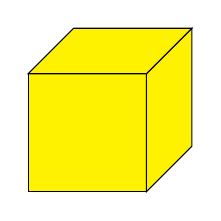
\begin{tikzpicture}
\pgfmathsetmacro{\cubex}{1.5}
\pgfmathsetmacro{\cubey}{1.5}
\pgfmathsetmacro{\cubez}{1.5}
\draw[black,fill=yellow] (0,0,0) -- ++(-\cubex,0,0) -- ++(0,-\cubey,0) -- ++(\cubex,0,0) -- cycle;
\draw[black,fill=yellow] (0,0,0) -- ++(0,0,-\cubez) -- ++(0,-\cubey,0) -- ++(0,0,\cubez) -- cycle;
\draw[black,fill=yellow] (0,0,0) -- ++(-\cubex,0,0) -- ++(0,0,-\cubez) -- ++(\cubex,0,0) -- cycle;
\end{tikzpicture}
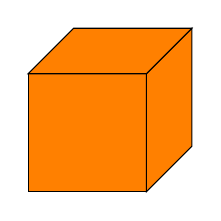
\begin{tikzpicture}
\pgfmathsetmacro{\cubex}{1.5}
\pgfmathsetmacro{\cubey}{1.5}
\pgfmathsetmacro{\cubez}{1.5}
\draw[black,fill=orange] (0,0,0) -- ++(-\cubex,0,0) -- ++(0,-\cubey,0) -- ++(\cubex,0,0) -- cycle;
\draw[black,fill=orange] (0,0,0) -- ++(0,0,-\cubez) -- ++(0,-\cubey,0) -- ++(0,0,\cubez) -- cycle;
\draw[black,fill=orange] (0,0,0) -- ++(-\cubex,0,0) -- ++(0,0,-\cubez) -- ++(\cubex,0,0) -- cycle;
\end{tikzpicture}
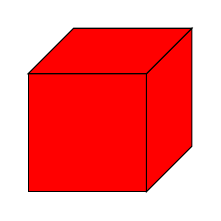
\begin{tikzpicture}
\pgfmathsetmacro{\cubex}{1.5}
\pgfmathsetmacro{\cubey}{1.5}
\pgfmathsetmacro{\cubez}{1.5}
\draw[black,fill=red] (0,0,0) -- ++(-\cubex,0,0) -- ++(0,-\cubey,0) -- ++(\cubex,0,0) -- cycle;
\draw[black,fill=red] (0,0,0) -- ++(0,0,-\cubez) -- ++(0,-\cubey,0) -- ++(0,0,\cubez) -- cycle;
\draw[black,fill=red] (0,0,0) -- ++(-\cubex,0,0) -- ++(0,0,-\cubez) -- ++(\cubex,0,0) -- cycle;
\end{tikzpicture}
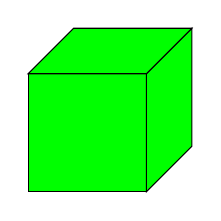
\begin{tikzpicture}
\pgfmathsetmacro{\cubex}{1.5}
\pgfmathsetmacro{\cubey}{1.5}
\pgfmathsetmacro{\cubez}{1.5}
\draw[black,fill=green] (0,0,0) -- ++(-\cubex,0,0) -- ++(0,-\cubey,0) -- ++(\cubex,0,0) -- cycle;
\draw[black,fill=green] (0,0,0) -- ++(0,0,-\cubez) -- ++(0,-\cubey,0) -- ++(0,0,\cubez) -- cycle;
\draw[black,fill=green] (0,0,0) -- ++(-\cubex,0,0) -- ++(0,0,-\cubez) -- ++(\cubex,0,0) -- cycle;
\end{tikzpicture}
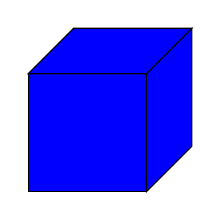
\begin{tikzpicture}
\pgfmathsetmacro{\cubex}{1.5}
\pgfmathsetmacro{\cubey}{1.5}
\pgfmathsetmacro{\cubez}{1.5}
\draw[black,fill=blue] (0,0,0) -- ++(-\cubex,0,0) -- ++(0,-\cubey,0) -- ++(\cubex,0,0) -- cycle;
\draw[black,fill=blue] (0,0,0) -- ++(0,0,-\cubez) -- ++(0,-\cubey,0) -- ++(0,0,\cubez) -- cycle;
\draw[black,fill=blue] (0,0,0) -- ++(-\cubex,0,0) -- ++(0,0,-\cubez) -- ++(\cubex,0,0) -- cycle;
\end{tikzpicture}
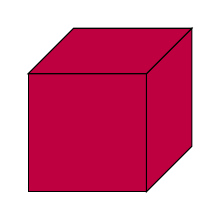
\begin{tikzpicture}
\pgfmathsetmacro{\cubex}{1.5}
\pgfmathsetmacro{\cubey}{1.5}
\pgfmathsetmacro{\cubez}{1.5}
\draw[black,fill=purple] (0,0,0) -- ++(-\cubex,0,0) -- ++(0,-\cubey,0) -- ++(\cubex,0,0) -- cycle;
\draw[black,fill=purple] (0,0,0) -- ++(0,0,-\cubez) -- ++(0,-\cubey,0) -- ++(0,0,\cubez) -- cycle;
\draw[black,fill=purple] (0,0,0) -- ++(-\cubex,0,0) -- ++(0,0,-\cubez) -- ++(\cubex,0,0) -- cycle;
\end{tikzpicture}
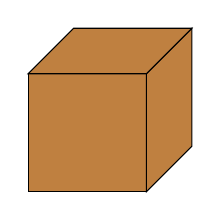
\begin{tikzpicture}
\pgfmathsetmacro{\cubex}{1.5}
\pgfmathsetmacro{\cubey}{1.5}
\pgfmathsetmacro{\cubez}{1.5}
\draw[black,fill=brown] (0,0,0) -- ++(-\cubex,0,0) -- ++(0,-\cubey,0) -- ++(\cubex,0,0) -- cycle;
\draw[black,fill=brown] (0,0,0) -- ++(0,0,-\cubez) -- ++(0,-\cubey,0) -- ++(0,0,\cubez) -- cycle;
\draw[black,fill=brown] (0,0,0) -- ++(-\cubex,0,0) -- ++(0,0,-\cubez) -- ++(\cubex,0,0) -- cycle;
\end{tikzpicture}

\begin{tikzpicture}
\pgfmathsetmacro{\cubex}{1.5}
\pgfmathsetmacro{\cubey}{1.5}
\pgfmathsetmacro{\cubez}{1.5}
\draw[black,fill=black] (0,0,0) -- ++(-\cubex,0,0) -- ++(0,-\cubey,0) -- ++(\cubex,0,0) -- cycle;
\draw[black,fill=black] (0,0,0) -- ++(0,0,-\cubez) -- ++(0,-\cubey,0) -- ++(0,0,\cubez) -- cycle;
\draw[black,fill=black] (0,0,0) -- ++(-\cubex,0,0) -- ++(0,0,-\cubez) -- ++(\cubex,0,0) -- cycle;
\end{tikzpicture}\\
\vspace{1cm}
\begin{itemize}
\item How many choices do you have? -- Well, 8.
\item Just to make it more complicated: in \textbf{bits} this is $log_2(8)=3$
\item Translated into binary code: \\ \small 000 001 010 100 011 110 101 111
\end{itemize}
\end{frame}

\subsection{Information and Language}
\begin{frame}{How does this relate to language?}
\hspace{3cm}
``Where is the coin?''
\includegraphics[width=1cm,height=1.5cm]{img/boy.png}
\center
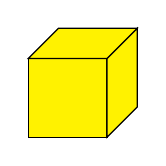
\begin{tikzpicture}
\pgfmathsetmacro{\cubex}{1}
\pgfmathsetmacro{\cubey}{1}
\pgfmathsetmacro{\cubez}{1}
\draw[black,fill=yellow] (0,0,0) -- ++(-\cubex,0,0) -- ++(0,-\cubey,0) -- ++(\cubex,0,0) -- cycle;
\draw[black,fill=yellow] (0,0,0) -- ++(0,0,-\cubez) -- ++(0,-\cubey,0) -- ++(0,0,\cubez) -- cycle;
\draw[black,fill=yellow] (0,0,0) -- ++(-\cubex,0,0) -- ++(0,0,-\cubez) -- ++(\cubex,0,0) -- cycle;
\end{tikzpicture}
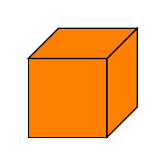
\begin{tikzpicture}
\pgfmathsetmacro{\cubex}{1}
\pgfmathsetmacro{\cubey}{1}
\pgfmathsetmacro{\cubez}{1}
\draw[black,fill=orange] (0,0,0) -- ++(-\cubex,0,0) -- ++(0,-\cubey,0) -- ++(\cubex,0,0) -- cycle;
\draw[black,fill=orange] (0,0,0) -- ++(0,0,-\cubez) -- ++(0,-\cubey,0) -- ++(0,0,\cubez) -- cycle;
\draw[black,fill=orange] (0,0,0) -- ++(-\cubex,0,0) -- ++(0,0,-\cubez) -- ++(\cubex,0,0) -- cycle;
\end{tikzpicture}
\begin{tikzpicture}
\pgfmathsetmacro{\cubex}{1}
\pgfmathsetmacro{\cubey}{1}
\pgfmathsetmacro{\cubez}{1}
\draw[black,fill=red] (0,0,0) -- ++(-\cubex,0,0) -- ++(0,-\cubey,0) -- ++(\cubex,0,0) -- cycle;
\node[yslant=0,anchor=center,opacity=1]  at (-0.3,-0.3,-0.3){\includegraphics[width=1cm,height=1cm]{img/coin.pdf}};
\draw[black,fill=red] (0,0,0) -- ++(0,0,-\cubez) -- ++(0,-\cubey,0) -- ++(0,0,\cubez) -- cycle;
\draw[black,fill=red] (0,0,0) -- ++(-\cubex,0,0) -- ++(0,0,-\cubez) -- ++(\cubex,0,0) -- cycle;
\end{tikzpicture}
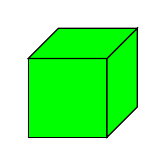
\begin{tikzpicture}
\pgfmathsetmacro{\cubex}{1}
\pgfmathsetmacro{\cubey}{1}
\pgfmathsetmacro{\cubez}{1}
\draw[black,fill=green] (0,0,0) -- ++(-\cubex,0,0) -- ++(0,-\cubey,0) -- ++(\cubex,0,0) -- cycle;
\draw[black,fill=green] (0,0,0) -- ++(0,0,-\cubez) -- ++(0,-\cubey,0) -- ++(0,0,\cubez) -- cycle;
\draw[black,fill=green] (0,0,0) -- ++(-\cubex,0,0) -- ++(0,0,-\cubez) -- ++(\cubex,0,0) -- cycle;
\end{tikzpicture}
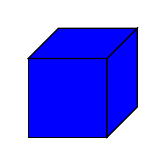
\begin{tikzpicture}
\pgfmathsetmacro{\cubex}{1}
\pgfmathsetmacro{\cubey}{1}
\pgfmathsetmacro{\cubez}{1}
\draw[black,fill=blue] (0,0,0) -- ++(-\cubex,0,0) -- ++(0,-\cubey,0) -- ++(\cubex,0,0) -- cycle;
\draw[black,fill=blue] (0,0,0) -- ++(0,0,-\cubez) -- ++(0,-\cubey,0) -- ++(0,0,\cubez) -- cycle;
\draw[black,fill=blue] (0,0,0) -- ++(-\cubex,0,0) -- ++(0,0,-\cubez) -- ++(\cubex,0,0) -- cycle;
\end{tikzpicture}
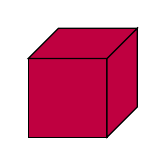
\begin{tikzpicture}
\pgfmathsetmacro{\cubex}{1}
\pgfmathsetmacro{\cubey}{1}
\pgfmathsetmacro{\cubez}{1}
\draw[black,fill=purple] (0,0,0) -- ++(-\cubex,0,0) -- ++(0,-\cubey,0) -- ++(\cubex,0,0) -- cycle;
\draw[black,fill=purple] (0,0,0) -- ++(0,0,-\cubez) -- ++(0,-\cubey,0) -- ++(0,0,\cubez) -- cycle;
\draw[black,fill=purple] (0,0,0) -- ++(-\cubex,0,0) -- ++(0,0,-\cubez) -- ++(\cubex,0,0) -- cycle;
\end{tikzpicture}
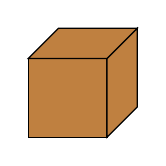
\begin{tikzpicture}
\pgfmathsetmacro{\cubex}{1}
\pgfmathsetmacro{\cubey}{1}
\pgfmathsetmacro{\cubez}{1}
\draw[black,fill=brown] (0,0,0) -- ++(-\cubex,0,0) -- ++(0,-\cubey,0) -- ++(\cubex,0,0) -- cycle;
\draw[black,fill=brown] (0,0,0) -- ++(0,0,-\cubez) -- ++(0,-\cubey,0) -- ++(0,0,\cubez) -- cycle;
\draw[black,fill=brown] (0,0,0) -- ++(-\cubex,0,0) -- ++(0,0,-\cubez) -- ++(\cubex,0,0) -- cycle;
\end{tikzpicture}

\begin{tikzpicture}
\pgfmathsetmacro{\cubex}{1}
\pgfmathsetmacro{\cubey}{1}
\pgfmathsetmacro{\cubez}{1}
\draw[black,fill=black] (0,0,0) -- ++(-\cubex,0,0) -- ++(0,-\cubey,0) -- ++(\cubex,0,0) -- cycle;
\draw[black,fill=black] (0,0,0) -- ++(0,0,-\cubez) -- ++(0,-\cubey,0) -- ++(0,0,\cubez) -- cycle;
\draw[black,fill=black] (0,0,0) -- ++(-\cubex,0,0) -- ++(0,0,-\cubez) -- ++(\cubex,0,0) -- cycle;
\end{tikzpicture}
\flushleft
\hspace{3cm}
\includegraphics[width=1cm,height=1.5cm]{img/girl.png}
\hspace{0.5cm}``In the \color{red}red \color{black}box''\\
\small
\begin{itemize}
\item The ``alphabet'' (here words) of the ``language'' they use does not need more than 8 colour adjectives to disambiguate:\\
\center
\vspace{0.1cm}
$\mathcal{A}=\{\color{yellow}yellow, \color{orange}orange, \color{red}red, \color{green}green, \color{blue}blue,\color{purple}purple, \color{brown}brown, \color{black}black\}$\\
\vspace{0.2cm}
\end{itemize}
\end{frame}

\begin{frame}{}
\small
Assume we play this game $n$ times. The probability of a coin being put into any of the boxes is $p(col)=\frac{1}{8}$. This is a \textit{random} and \textit{uniform} distribution of probabilities. \\
\vspace{0.2cm}
\includegraphics[width=1cm,height=1.5cm]{img/girl.png}
\hspace{0.5cm}``In the \color{red}red/\color{green}green/\color{blue}blue/ \color{yellow}yellow/\color{purple} purple/\color{brown} brown/\color{black}black ... box''\\
\vspace{0.2cm}
\flushleft
The probabilities of words occurring in the \textbf{girl's language} will match this distribution in the limit, i.e. as $n\rightarrow\infty$.\\
\vspace{0.5cm}
\includegraphics[width=0.3\textwidth]{img/colgame80.pdf}
\includegraphics[width=0.3\textwidth]{img/colgame800.pdf}
\includegraphics[width=0.3\textwidth]{img/colgame80K.pdf}\\
\vspace{0.5cm}
\end{frame}

\begin{frame}{}
\begin{block}{The bottom line is:}
Notice how in this simple communication game, the probabilities of occurrences of \textbf{words} (color adjectives) start to reflect the probabilities of occurrences of \textbf{situations} in the ``real world'' (coins in boxes) -- \textbf{if communication is truthful}.  
\end{block}
\vspace{0.5cm}
However, is this relevant to ``real'' natural language?
\end{frame}

\begin{frame}{Example: Frequencies of Mountain Names}
\centering
\includegraphics[width=0.9\textwidth]{img/derungs2.png}\\
\flushleft
\footnotesize
\color{gray}
Derungs \& Samard\v{z}i\'{c} (2017). Are prominent mountains frequently mentioned in text?
\end{frame}

\begin{frame}{}
\vspace{0.5cm}
\centering
\includegraphics[width=1\textwidth]{img/derungs.png}
\flushleft
\small
The frequency of occurrence of so-called toponyms (in this case names of famous mountains) in texts is significantly correlated with measures of spatial salience (e.g. height), especially if a text is written in a location close-by.\\
\vspace{0.2cm}
Hence, this is an example of how \textbf{real world salience} is reflected in \textbf{probabilities of occurrence in language}.
\end{frame}

\begin{frame}{What if we change the game?}
\hspace{3cm}
``Where is the coin?''
\includegraphics[width=1cm,height=1.5cm]{img/boy.png}\\
\vspace{0.5cm}
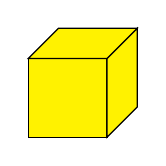
\begin{tikzpicture}
\pgfmathsetmacro{\cubex}{1}
\pgfmathsetmacro{\cubey}{1}
\pgfmathsetmacro{\cubez}{1}
\draw[black,fill=yellow] (0,0,0) -- ++(-\cubex,0,0) -- ++(0,-\cubey,0) -- ++(\cubex,0,0) -- cycle;
\draw[black,fill=yellow] (0,0,0) -- ++(0,0,-\cubez) -- ++(0,-\cubey,0) -- ++(0,0,\cubez) -- cycle;
\draw[black,fill=yellow] (0,0,0) -- ++(-\cubex,0,0) -- ++(0,0,-\cubez) -- ++(\cubex,0,0) -- cycle;
\end{tikzpicture}
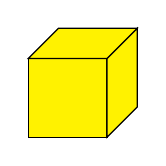
\begin{tikzpicture}
\pgfmathsetmacro{\cubex}{1}
\pgfmathsetmacro{\cubey}{1}
\pgfmathsetmacro{\cubez}{1}
\draw[black,fill=yellow] (0,0,0) -- ++(-\cubex,0,0) -- ++(0,-\cubey,0) -- ++(\cubex,0,0) -- cycle;
\draw[black,fill=yellow] (0,0,0) -- ++(0,0,-\cubez) -- ++(0,-\cubey,0) -- ++(0,0,\cubez) -- cycle;
\draw[black,fill=yellow] (0,0,0) -- ++(-\cubex,0,0) -- ++(0,0,-\cubez) -- ++(\cubex,0,0) -- cycle;
\end{tikzpicture}
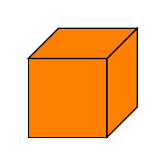
\begin{tikzpicture}
\pgfmathsetmacro{\cubex}{1}
\pgfmathsetmacro{\cubey}{1}
\pgfmathsetmacro{\cubez}{1}
\draw[black,fill=orange] (0,0,0) -- ++(-\cubex,0,0) -- ++(0,-\cubey,0) -- ++(\cubex,0,0) -- cycle;
\draw[black,fill=orange] (0,0,0) -- ++(0,0,-\cubez) -- ++(0,-\cubey,0) -- ++(0,0,\cubez) -- cycle;
\draw[black,fill=orange] (0,0,0) -- ++(-\cubex,0,0) -- ++(0,0,-\cubez) -- ++(\cubex,0,0) -- cycle;
\end{tikzpicture}
\begin{tikzpicture}
\pgfmathsetmacro{\cubex}{1}
\pgfmathsetmacro{\cubey}{1}
\pgfmathsetmacro{\cubez}{1}
\draw[black,fill=red] (0,0,0) -- ++(-\cubex,0,0) -- ++(0,-\cubey,0) -- ++(\cubex,0,0) -- cycle;
\node[yslant=0,anchor=center,opacity=1]  at (-0.3,-0.3,-0.3){\includegraphics[width=1cm,height=1cm]{img/coin.pdf}};
\draw[black,fill=red] (0,0,0) -- ++(0,0,-\cubez) -- ++(0,-\cubey,0) -- ++(0,0,\cubez) -- cycle;
\draw[black,fill=red] (0,0,0) -- ++(-\cubex,0,0) -- ++(0,0,-\cubez) -- ++(\cubex,0,0) -- cycle;
\end{tikzpicture}
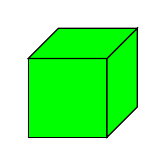
\begin{tikzpicture}
\pgfmathsetmacro{\cubex}{1}
\pgfmathsetmacro{\cubey}{1}
\pgfmathsetmacro{\cubez}{1}
\draw[black,fill=green] (0,0,0) -- ++(-\cubex,0,0) -- ++(0,-\cubey,0) -- ++(\cubex,0,0) -- cycle;
\draw[black,fill=green] (0,0,0) -- ++(0,0,-\cubez) -- ++(0,-\cubey,0) -- ++(0,0,\cubez) -- cycle;
\draw[black,fill=green] (0,0,0) -- ++(-\cubex,0,0) -- ++(0,0,-\cubez) -- ++(\cubex,0,0) -- cycle;
\end{tikzpicture}
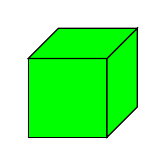
\begin{tikzpicture}
\pgfmathsetmacro{\cubex}{1}
\pgfmathsetmacro{\cubey}{1}
\pgfmathsetmacro{\cubez}{1}
\draw[black,fill=green] (0,0,0) -- ++(-\cubex,0,0) -- ++(0,-\cubey,0) -- ++(\cubex,0,0) -- cycle;
\draw[black,fill=green] (0,0,0) -- ++(0,0,-\cubez) -- ++(0,-\cubey,0) -- ++(0,0,\cubez) -- cycle;
\draw[black,fill=green] (0,0,0) -- ++(-\cubex,0,0) -- ++(0,0,-\cubez) -- ++(\cubex,0,0) -- cycle;
\end{tikzpicture}
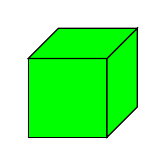
\begin{tikzpicture}
\pgfmathsetmacro{\cubex}{1}
\pgfmathsetmacro{\cubey}{1}
\pgfmathsetmacro{\cubez}{1}
\draw[black,fill=green] (0,0,0) -- ++(-\cubex,0,0) -- ++(0,-\cubey,0) -- ++(\cubex,0,0) -- cycle;
\draw[black,fill=green] (0,0,0) -- ++(0,0,-\cubez) -- ++(0,-\cubey,0) -- ++(0,0,\cubez) -- cycle;
\draw[black,fill=green] (0,0,0) -- ++(-\cubex,0,0) -- ++(0,0,-\cubez) -- ++(\cubex,0,0) -- cycle;
\end{tikzpicture}
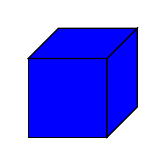
\begin{tikzpicture}
\pgfmathsetmacro{\cubex}{1}
\pgfmathsetmacro{\cubey}{1}
\pgfmathsetmacro{\cubez}{1}
\draw[black,fill=blue] (0,0,0) -- ++(-\cubex,0,0) -- ++(0,-\cubey,0) -- ++(\cubex,0,0) -- cycle;
\draw[black,fill=blue] (0,0,0) -- ++(0,0,-\cubez) -- ++(0,-\cubey,0) -- ++(0,0,\cubez) -- cycle;
\draw[black,fill=blue] (0,0,0) -- ++(-\cubex,0,0) -- ++(0,0,-\cubez) -- ++(\cubex,0,0) -- cycle;
\end{tikzpicture}
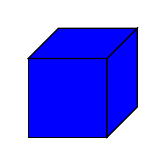
\begin{tikzpicture}
\pgfmathsetmacro{\cubex}{1}
\pgfmathsetmacro{\cubey}{1}
\pgfmathsetmacro{\cubez}{1}
\draw[black,fill=blue] (0,0,0) -- ++(-\cubex,0,0) -- ++(0,-\cubey,0) -- ++(\cubex,0,0) -- cycle;
\draw[black,fill=blue] (0,0,0) -- ++(0,0,-\cubez) -- ++(0,-\cubey,0) -- ++(0,0,\cubez) -- cycle;
\draw[black,fill=blue] (0,0,0) -- ++(-\cubex,0,0) -- ++(0,0,-\cubez) -- ++(\cubex,0,0) -- cycle;
\end{tikzpicture}
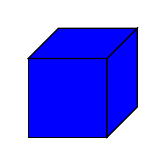
\begin{tikzpicture}
\pgfmathsetmacro{\cubex}{1}
\pgfmathsetmacro{\cubey}{1}
\pgfmathsetmacro{\cubez}{1}
\draw[black,fill=blue] (0,0,0) -- ++(-\cubex,0,0) -- ++(0,-\cubey,0) -- ++(\cubex,0,0) -- cycle;
\draw[black,fill=blue] (0,0,0) -- ++(0,0,-\cubez) -- ++(0,-\cubey,0) -- ++(0,0,\cubez) -- cycle;
\draw[black,fill=blue] (0,0,0) -- ++(-\cubex,0,0) -- ++(0,0,-\cubez) -- ++(\cubex,0,0) -- cycle;
\end{tikzpicture}
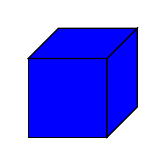
\begin{tikzpicture}
\pgfmathsetmacro{\cubex}{1}
\pgfmathsetmacro{\cubey}{1}
\pgfmathsetmacro{\cubez}{1}
\draw[black,fill=blue] (0,0,0) -- ++(-\cubex,0,0) -- ++(0,-\cubey,0) -- ++(\cubex,0,0) -- cycle;
\draw[black,fill=blue] (0,0,0) -- ++(0,0,-\cubez) -- ++(0,-\cubey,0) -- ++(0,0,\cubez) -- cycle;
\draw[black,fill=blue] (0,0,0) -- ++(-\cubex,0,0) -- ++(0,0,-\cubez) -- ++(\cubex,0,0) -- cycle;
\end{tikzpicture}
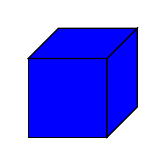
\begin{tikzpicture}
\pgfmathsetmacro{\cubex}{1}
\pgfmathsetmacro{\cubey}{1}
\pgfmathsetmacro{\cubez}{1}
\draw[black,fill=blue] (0,0,0) -- ++(-\cubex,0,0) -- ++(0,-\cubey,0) -- ++(\cubex,0,0) -- cycle;
\draw[black,fill=blue] (0,0,0) -- ++(0,0,-\cubez) -- ++(0,-\cubey,0) -- ++(0,0,\cubez) -- cycle;
\draw[black,fill=blue] (0,0,0) -- ++(-\cubex,0,0) -- ++(0,0,-\cubez) -- ++(\cubex,0,0) -- cycle;
\end{tikzpicture}
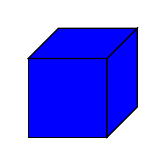
\begin{tikzpicture}
\pgfmathsetmacro{\cubex}{1}
\pgfmathsetmacro{\cubey}{1}
\pgfmathsetmacro{\cubez}{1}
\draw[black,fill=blue] (0,0,0) -- ++(-\cubex,0,0) -- ++(0,-\cubey,0) -- ++(\cubex,0,0) -- cycle;
\draw[black,fill=blue] (0,0,0) -- ++(0,0,-\cubez) -- ++(0,-\cubey,0) -- ++(0,0,\cubez) -- cycle;
\draw[black,fill=blue] (0,0,0) -- ++(-\cubex,0,0) -- ++(0,0,-\cubez) -- ++(\cubex,0,0) -- cycle;
\end{tikzpicture}
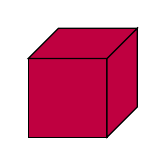
\begin{tikzpicture}
\pgfmathsetmacro{\cubex}{1}
\pgfmathsetmacro{\cubey}{1}
\pgfmathsetmacro{\cubez}{1}
\draw[black,fill=purple] (0,0,0) -- ++(-\cubex,0,0) -- ++(0,-\cubey,0) -- ++(\cubex,0,0) -- cycle;
\draw[black,fill=purple] (0,0,0) -- ++(0,0,-\cubez) -- ++(0,-\cubey,0) -- ++(0,0,\cubez) -- cycle;
\draw[black,fill=purple] (0,0,0) -- ++(-\cubex,0,0) -- ++(0,0,-\cubez) -- ++(\cubex,0,0) -- cycle;
\end{tikzpicture}
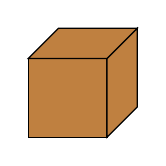
\begin{tikzpicture}
\pgfmathsetmacro{\cubex}{1}
\pgfmathsetmacro{\cubey}{1}
\pgfmathsetmacro{\cubez}{1}
\draw[black,fill=brown] (0,0,0) -- ++(-\cubex,0,0) -- ++(0,-\cubey,0) -- ++(\cubex,0,0) -- cycle;
\draw[black,fill=brown] (0,0,0) -- ++(0,0,-\cubez) -- ++(0,-\cubey,0) -- ++(0,0,\cubez) -- cycle;
\draw[black,fill=brown] (0,0,0) -- ++(-\cubex,0,0) -- ++(0,0,-\cubez) -- ++(\cubex,0,0) -- cycle;
\end{tikzpicture}

\begin{tikzpicture}
\pgfmathsetmacro{\cubex}{1}
\pgfmathsetmacro{\cubey}{1}
\pgfmathsetmacro{\cubez}{1}
\draw[black,fill=black] (0,0,0) -- ++(-\cubex,0,0) -- ++(0,-\cubey,0) -- ++(\cubex,0,0) -- cycle;
\draw[black,fill=black] (0,0,0) -- ++(0,0,-\cubez) -- ++(0,-\cubey,0) -- ++(0,0,\cubez) -- cycle;
\draw[black,fill=black] (0,0,0) -- ++(-\cubex,0,0) -- ++(0,0,-\cubez) -- ++(\cubex,0,0) -- cycle;
\end{tikzpicture}
\flushleft
\hspace{3cm}
\includegraphics[width=1cm,height=1.5cm]{img/girl.png}
\hspace{0.5cm}``In the \color{red}red \color{black}box''\\
\small
\begin{itemize}
\item The ``alphabet'' has \textbf{not} changed:\\
\center
\vspace{0.1cm}
$\mathcal{A}=\{\color{yellow}yellow, \color{orange}orange, \color{red}red, \color{green}green, \color{blue}blue,\color{purple}purple, \color{brown}brown, \color{black}black\}$\\
\vspace{0.2cm}
\end{itemize}
\end{frame}

\begin{frame}{}
\small
However, the probabilities of boxes/colours has changed: $p(blue)=\frac{6}{16}$, $p(green)=\frac{3}{16}$, $p(yellow)=\frac{2}{16}$, $p(purple)=\frac{1}{16}$, etc.  \\
\vspace{0.2cm}
\includegraphics[width=1cm,height=1.5cm]{img/girl.png}
\hspace{0.5cm}``In the \color{red}red, \color{green}green, \color{blue}blue, \color{blue}blue \color{yellow}yellow, \color{purple} purple, \color{blue}blue,\color{black} ... box''\\
\vspace{0.2cm}
\flushleft
Again, this will be reflected in the \textbf{girl's language production}.\\
\vspace{0.5cm}
\includegraphics[width=0.3\textwidth]{img/colgame160.pdf}
\includegraphics[width=0.3\textwidth]{img/colgame1600.pdf}
\includegraphics[width=0.3\textwidth]{img/colgame160K.pdf}
\end{frame}

\begin{frame}{Comparing language production}
\small
If we play the two games the same number of times $n$, we will get the same two languages \textbf{$L_A$} and $L_B$ in terms of \textbf{word types} (8 in this case), and the number of \textbf{word tokens} (10K in this case).\\
\vspace{0.5cm} 
However, the \textbf{distributions} of \textbf{word token} counts differ!\\  
\center
\includegraphics[width=0.4\textwidth]{img/colgameA10K.pdf}
\includegraphics[width=0.4\textwidth]{img/colgameB10K.pdf}
\end{frame}

\begin{frame}{Crucially: Certainty and Uncertainty in the Game}
\small
Note that in $L_A$ there is \textbf{more uncertainty}, \textbf{more choice/possibility} than in $L_B$. If we had to take a guess what the girl says next, then in $L_A$ we have a uniform chance of $\frac{1}{8}=0.125$ of being right, whereas in $L_B$ we have a better chance of $\frac{6}{16}=\frac{3}{8}=0.375$ if we guess ``blue''.\\
\centering
\vspace{0.5cm} 
\includegraphics[width=0.4\textwidth]{img/colgameA10K.pdf}
\includegraphics[width=0.4\textwidth]{img/colgameB10K.pdf}
\end{frame}


\section{Section 3: Measuring Entropy}

{
\setbeamertemplate{sidebar right}{}
\begin{frame}
\title{Section 3: Measuring Entropy} %Titel
\newcommand{\titelbild}{{\color{grau}\rule{\textwidth}{70mm}}\\[-0.4cm]{\color{rot}\rule{\textwidth}{5mm}}} %statt grauer Box ein Deckblattbild einf�gen und die rote Linie nach oben versetzen, hier um 0.35cm
\maketitle
\end{frame}
}

\begin{frame}{How can we measure this difference in the distributions?}
Claude Shannon came up with a measure for this difference in "A mathematical theory of communication" (1948). He called it the \textbf{entropy H}, after the concept known from thermodynamics.
\vspace{0.5cm} 
\center
\includegraphics[width=0.7\textwidth]{img/shannon.jpg}\\
\vspace{0.5cm}
\flushleft 
Note that there can be different notations and versions of that formular, which is confusing at times.
\end{frame}

\subsection{Definition}
\begin{frame}{A more precise formulation\\ \small (See also Cover \& Thomas, 2006)}
Assume that
\begin{itemize}
\item $X$ is a \textit{discrete random variable}, drawn from an alphabet of possible values \textbf{$\mathcal{X}=\{x_1,x_2,...,x_N\}$}, where $N=|\mathcal{X}|$ \\
\vspace{0.2cm} 
\small Example: The ``alphabet'' or set of colour adjectives, e.g. $\mathcal{A}=\{yellow,orange,red,green,blue,purple,brown,black\}$, with $N=8$

\item \normalsize The \textit{probability mass function} is defined by $p(x)=Pr\{X=x\}, x\in \mathcal{X}$\\
\small
\vspace{0.2cm}
Example: each word type is assigned a probability, e.g. in $L_B$ $p(blue)=\frac{6}{16}$, $p(green)=\frac{3}{16}$ etc. 
\end{itemize}
\end{frame}

\begin{frame}{A more precise formulation}
Given these definitions, the entropy is then defined as
\begin{equation}
H(X)=-\sum_{x\in \mathcal{X}} p(x) \log p(x).
\end{equation}
Notes:
\small
\begin{itemize}
\item The logarithm is typically taken to the base 2, i.e. giving bits of information. We will henceforth indicate this explicitely. 
\item In the original article by Shannon, there was also a positive constant $K$ before the summation sign, but henceforth it was mostly assumed to be $1$, and hence dropped.
\item There are many alternative - notationally different, but conceptually equivalent - formulations of the entropy. Shannon, for instance, used $H(p_1,p_2,...,p_N)$, which is mostly shortened to $H(X)$.
\end{itemize}
\end{frame}

\begin{frame}{Let's look at the component parts}
\begin{equation}
H(X)={\color{red}-}\sum_{x\in \mathcal{X}} p(x) {\color{red}\log_2 p(x)}.
\end{equation}
\small
\begin{itemize}
\item {\color{red}$-\log_2 p(x)$} is the \textbf{information content} of a unit $x$ (word type in the case of the box game). In the case where units are independent of each other, the probability is essentially a normalized frequency. The frequency of a unit determines how much information it carries. The minus sign is just there to not get a negative value, since the logarithm of probabilities ($0 < p(x) < 1$) is negative (except for $p(x) = 1$, for which it is $0$).\\
\vspace{0.2cm}
For example, in $L_B$ the word type ``blue'' occurs ca. 3750 times in 10000 tokens, and its information content is $-\log_2(\frac{3750}{10000})\sim 1.42$ bits. The word type "orange", on the other hand, occurs ca. 625 times in 10000 tokens, its information content is $-\log_2(\frac{625}{10000})\sim 4$ bits. Hence, the word type ``orange'' has higher information content.    
\end{itemize}
\end{frame}

\begin{frame}{Let's look at the component parts}
\begin{equation}
H(X)=-{\color{red}\sum_{x\in \mathcal{X}} p(x)} \log_2 p(x)
\end{equation}
\small
\begin{itemize}
\item The summation part of the equation means that we multiply the information content of each element $x$ with its probability $p(x)$, and sum over all of them. Note that multiplying all elements with their probabilities just means that we take the average. \\
\normalsize
\vspace{0.5cm}
\textbf{Hence, the entropy $H(X)$ can be seen as the \textbf{average information content} of information encoding units, i.e. adjective word types in the case of the box game.}     
\end{itemize}
\end{frame}

\subsection{Application to Languages}
\begin{frame}{Let's apply this to Languages A and B}
\small
For reasons of simplicity let's take the expected values and not actual counts:\\
\footnotesize
\begin{equation}
H(L_A)=-(\frac{1}{8} \times \log_2(\frac{1}{8})+\frac{1}{8} \times \log_2(\frac{1}{8})+ ... + \frac{1}{8} \times \log_2(\frac{1}{8}))=\textbf{3}\footnote{Note: the case where we have a uniform distribution of probabilities, i.e. all events (adjectives here) are exactly equally likely, is the \textbf{maximum entropy} case. In this case, the equation simplifies to $log_2 (N)$. Such that here we have log_2(8)=3.}
\end{equation}
\begin{equation}
H(L_B)=-(\frac{6}{16} \times \log_2(\frac{6}{16})+\frac{3}{16} \times \log_2(\frac{3}{16})+ ... + \frac{1}{16} \times \log_2(\frac{1}{16}))=\textbf{2.61}
\end{equation}
\center
\vspace{0.5cm} 
\includegraphics[width=0.4\textwidth]{img/colgameA10K.pdf}
\includegraphics[width=0.4\textwidth]{img/colgameB10K.pdf}
\end{frame}

\begin{frame}{}
\small
\begin{itemize}
\item Word types in Language $A$ carry \textbf{3 bits} of information on average, whereas word types in Language $B$ carry only \textbf{2.61 bits}.
\item Note that 3 bits is actually the \textbf{maximum entropy} possible for a language with 8 word types, since this is the case with uniform probabilities $\frac{1}{8}$. 
\item The \textbf{minimum entropy} would be $0$, namely in the case where only 1 word type is used, since $\log_2(\frac{8}{8})=0$. 
\end{itemize}
\vspace{0.5cm}
\center 
\includegraphics[width=0.4\textwidth]{img/colgameA10K.pdf}
\includegraphics[width=0.4\textwidth]{img/colgameB10K.pdf}
\end{frame}

\section{Section 4: Two Problems and Solutions}

{
\setbeamertemplate{sidebar right}{}
\begin{frame}
\title{Section 4: Two Problems and Solutions} %Titel
\newcommand{\titelbild}{{\color{grau}\rule{\textwidth}{70mm}}\\[-0.4cm]{\color{rot}\rule{\textwidth}{5mm}}} %statt grauer Box ein Deckblattbild einf�gen und die rote Linie nach oben versetzen, hier um 0.35cm
\maketitle
\end{frame}
}

\begin{frame}{}
\flushleft
That's great! We have a tool at hand to measure the\\ information encoding potential of any communicative (and non-communicative) system!\\
\center
\includegraphics[width=0.6\textwidth]{img/shannon3.pdf}
\end{frame}

\begin{frame}{}
\begin{block}{Two Major Problems}
\large
\begin{enumerate}
\item What is an information encoding ``unit'' in the first place - and how does this effect the results?
\item What is the ``real'' probability of letters, words, sentences, or symbols more generally? 
\end{enumerate}
\end{block}
\end{frame}

\begin{frame}{}
\begin{block}{Problem 1}
We will deal with the problem of information encoding units and their impact on the results of entropy estimation in the Exercise Sheet for Tutorial Week 1.
\end{block}
\end{frame}

\begin{frame}{}
\begin{block}{Problem 2a: What's the ``real'' probability?}
The probabilities of letters, words, phrases, etc. depend on the \textbf{corpus size}, and so does the entropy $H(X)$.
\end{block}
\vspace{0.5cm}
\includegraphics[width=0.3\textwidth]{img/eng10words.pdf}\includegraphics[width=0.3\textwidth]{img/eng100words.pdf}
\includegraphics[width=0.3\textwidth]{img/eng1000words.pdf}\\
\vspace{0.5cm}
\small
Figure. Frequency distributions and word type entropies for the English UDHR according to the first 10, 100, 1000 word tokens.
\end{frame}

\begin{frame} {}
\begin{block}{Possible Solution for Problem 2a}
\small
Get better entropy estimators (e.g. Hausser \& Strimmer 2014 via R package \textit{entropy}), and estimate the text size for which the entropy stabilizes.
\end{block}
\vspace{0.5cm}
\includegraphics[width=1\textwidth]{img/Hconv.pdf}\\
\footnotesize
\color{gray}
Bentz et al. (2017). The entropy of words - learnability and expressivity across more than 1000 languages. \textit{Entropy}.
\end{frame}

\begin{frame}{}
\begin{block}{Problem 2b: What's the ``real'' probability?}
Letters, words, phrases etc. are \textbf{not} drawn randomly and \textbf{independently} from one another. Instead, the \textbf{co-text} and \textbf{context} results in \textbf{conditional probabilities and entropies}.\\
\end{block}
\vspace{0.2cm}
\color{black}
Conditional probability: $p(y|x)=\frac{p(x,y)}{p(x)}$\\
\vspace{0.2cm}
Example for the first 100 tokens of the English UDHR:\\
\vspace{0.2cm} 
While the simple unigram probability of ``the'' is\\
$p(the)=\frac{9}{100}=\textbf{0.09}$,\\
\vspace{0.2cm}
the probability of ``the'' conditioned on ``of'' is
$p(the|of)=\frac{p(of,the)}{p(of)}=\frac{\frac{4}{100}}{\frac{10}{100}}=\frac{4}{10}=\textbf{0.4}$.
\end{frame}

\begin{frame} {}
\begin{block}{Possible Solution for Problem 2b}
\begin{itemize}
\item Estimate \textbf{n-gram} (bigram, trigram, etc.) entropies instead of unigram entropies. However, this soon requires very big corpora as $n$ increases. This is a fundamental problem often referred to as \textit{data sparsity}.
\item Estimate the \textbf{entropy rate} \textit{h}, which reflects the growth of the entropy with the length of a string, i.e. \textit{n} in our case (Cover \& Thomas, 2006, p. 74). 
\end{itemize}
\end{block}
\end{frame}

\section{Summary}

%Section beginning slide
{
\setbeamertemplate{sidebar right}{}
\begin{frame}
\title{Summary} %Titel
\newcommand{\titelbild}{{\color{grau}\rule{\textwidth}{70mm}}\\[-0.4cm]{\color{rot}\rule{\textwidth}{5mm}}} %statt grauer Box ein Deckblattbild einf�gen und die rote Linie nach oben versetzen, hier um 0.35cm
\maketitle
\end{frame}
}

\begin{frame}{Summary}
\begin{itemize}
\item Information theory gives us an understanding of the fundamentals of \textbf{information encoding and decoding}. Communication also harnesses these processes.\vspace{0.2cm}
\item The information contained in a string of symbols can be \textbf{defined mathematically}, and \textbf{measured empirically}.\vspace{0.2cm}
\item Information contained in a communication system might reflect information contained in the real world.\vspace{0.2cm}
\item Entropy is a measure of the \textbf{information encoding potential} of a symbol system. 
\end{itemize}  
\end{frame}


\section{References}

{
\setbeamertemplate{sidebar right}{}
\begin{frame}
\title{References} %Titel
\newcommand{\titelbild}{{\color{grau}\rule{\textwidth}{70mm}}\\[-0.4cm]{\color{rot}\rule{\textwidth}{5mm}}} %statt grauer Box ein Deckblattbild einf�gen und die rote Linie nach oben versetzen, hier um 0.35cm
\maketitle
\end{frame}
}

\begin{frame}{References} %dritte Folie
\small
Bentz, Christian, Alikaniotis, Dimitrios, Ferrer-i-Cancho, Ramon \& Cysouw, Michael (2017). The entropy of words - learnability and expressivity across more than 1000 languages. \textit{Entropy}.
\\ 
\vspace{0.2cm}
Cover, Thomas M. \& Thomas, Joy A. (2006). \textit{Elements of Information Theory.} New Jersey: Wiley \& Sons.
\\
\vspace{0.2cm}
Derungs, Curdin \& Samard\v{z}i\'{c}, Tanja (2017). Are prominent mountains frequently mentioned in text? Exploring the spatial expressiveness of text frequency. \textit{International Journal of Geographical Information Science}.
\\ 
\vspace{0.2cm}
Lemons, Don S. (2013). \textit{A student's guide to entropy}. Cambridge: Cambridge University Press.
\\ 
\vspace{0.2cm}
Shannon, Claude E. \& Weaver, Warren (1949). \textit{The mathematical theory of communication.} Chicago: University of Illinois Press.
\end{frame}


%Letzte Slide
%Letzte Slide
{
\setbeamertemplate{sidebar right}{}
\begin{frame}[c] %R�ckfolie
\colorbox{rot}{\parbox{\textwidth}{\centering\vspace*{1.5cm} \parbox{12cm}{\color{white} {\huge Thank You.} 
\small
\bigskip \\ {\bf Contact:} \bigskip \\ {\fakult}\\ \fbname\\ Dr. Christian Bentz \\
SFS Wilhelmstra\ss e 19-23, Room 1.24\\
chris@christianbentz.de\\
Office hours: \\
During term: Wednesdays 10-11am\\
Out of term: arrange via e-mail
}
\vspace*{1.5cm}}}
\end{frame}
}
%------------------------------------------------------
\end{document}